\documentclass[12pt, a4paper]{article}

% --- Pacotes Básicos ---
\usepackage[utf8]{inputenc}
\usepackage{graphicx}
\usepackage[T1]{fontenc}
\usepackage[main=brazilian, english]{babel}
\usepackage{indentfirst}
\usepackage{geometry}
\geometry{left=3cm, top=3cm, right=2cm, bottom=2cm}

% --- Informações do Documento ---
\title{Estudos em Criptografia Pós-Quântica}
\author{Erickson G. Müller}
\date{\today}

\begin{document}
\maketitle
\thispagestyle{empty} % primeira página não tem número.


\section{Criptografia}
A criptografia é o processo de transformar uma mensagem legível em uma mensagem cifrada. Essa mensagem só poderia ser descriptografada com o uso de uma chave criptográfica, garantindo assim confidencialidade à mensagem. Também é usada para autenticidade, por meio da assinatura digital.Uma chave criptográfica pode ser simétrica ou assimétrica.

\subsection{Criptografia Simétrica}
Duas partes (A e B) querem se comunicar através de um canal aberto (inseguro). A criptografa a mensagem antes de entrar no canal e B deve descriptografar a mensagem após sair do canal. Portanto, temos duas funções, a de criptografar e a de descriptografar. Enquanto a mensagem criptografada passa por um canal inseguro, a chave para rodar as funções é passada por um canal seguro.

\begin{center}
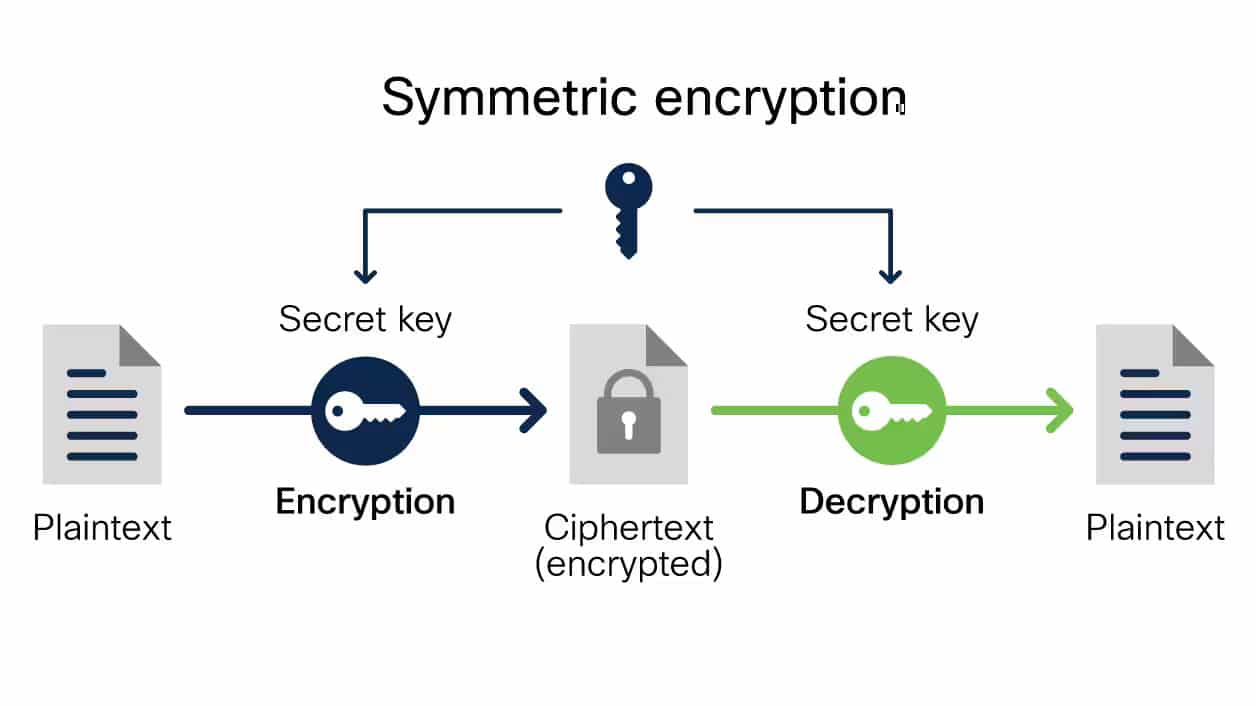
\includegraphics[scale=0.25]{images/symmetric-encryption-816386435.jpg}
\end{center}

\subsection{Criptografia Assimétrica}
A criptografia assimétrica, ou criptografia de chave pública, usa duas chaves. Para confidencialidade, a informação é criptografada com a chave pública do destinatário e só pode ser descriptografada pelo destinatário usando a própria chave privada. Para autenticidade e integridade, utiliza-se a assinatura digital em que a mensagem é assinada com a chave privada do remetente e a verificação é feita com a chave pública do remetente.

%\section{AES}
\section{Criptografia Baseada em Hash}
Os algoritmos criptográficos baseados em HASH são unidirecionais. Eles nunca são descriptografados pois hashs são funções irreversíveis, a verificação acontece recalculando o hash da mensagem e comparando os resumos.

\subsection{Funções Hash}
A função hash $H$, de $n$ bits, mapeia uma mensagem binária de grande tamanho (notação: $x = \{0,1\}^{\leq L}$ ou $x = \{0,1\}^{*}$) em um resumo criptográfico $H(x)$ de menor tamanho ($n = 256$). O hash consegue ser computado com mais eficiência que a mensagem inteira. A descrição da função hash é pública e fixa, portanto $H$ não tem chaves privadas.

As funções hashes possuem três propriedades de segurança:
\begin{itemize}
	\item \textbf{Preimage Resistance:} tendo um hash criptográfico $y$, é impossível encontrar a mensagem $x$ para a função $H(x) = y$.
	\item \textbf{Second Preimage Resistance:} tendo verificado um bit $x$ da mensagem, é impossível encontrar outro bit $x'$ com $x\neq x'$ e $H(x) = H(x')$
	\item \textbf{Collision Resistance:} impossível encontrar duas mensagens $x$ e $x'$ que possuam o mesmo resumo criptográfico.
\end{itemize}
Com $x \in \{0,1\}^*$ e $y \in \{0,1\}^n$.

Preimage resistance e $2^{nd}$ preimage resistance levam $2^n$ operações para serem quebradas com computação clássica, a computação quântica do Algoritmo de Grover consegue reduzir esse número para $2^{n/2}$. Já a identificação de colisão leva $2^{n/2}$ tanto com computadores clássicos quanto quânticos.


\section{Assinatura}
Um esquema de assinatura consiste em três algoritmos:
\begin{enumerate}
	\item \textbf{Geração das chaves:} o sistema gera o par de chaves matematicamente ligadas. A chave privada é mantida com o proprietário e a chave pública é disponibilizada publicamente para verificar as assinaturas.
	\item \textbf{Geração da assinatura:} o remetente utiliza sua chave privada e a mensagem a ser assinada para calcular a assinatura ($\sigma$).
	\item \textbf{Verificação da assinatura:} quem recebe a mensagem usa a chave pública do rementente para verificar a assinatura da mensagem. O cálculo é feito usando a assinatura, a chave pública e a mensagem.
\end{enumerate}

Para não assinar a mensagem inteira, o que demandaria excesso de processamento, a mensagem é passada por uma função de Hash que gera um resumo criptográfico de tamanho fixo (ver SHA-256). A chave privada assina apenas esse resumo, se a mensagem for alterada, o hash é alterado e a assinatura é inválida.

Como funções Hash são unidirecionais, só podem ser quebrados através de brute-force. Um computador quântico consegue acelerar esse processo, portanto, foram desenvolvidos algoritmos de criptografia baseados em HASH que são resistentes ao cenário pós-quântico. Para isso, usam chaves públicas e assinaturas exageradamente longas.

\subsection{Assinatura de Lamport}
One-Time Signature Scheme




\subsection{WOTS}
\subsection{Merkle Trees}
\subsection{XMSS (NIST SP 800-208)}

%\section{RSA}
%\section{Curvas Elípticas}

\section{Algoritmo de SHOR}
É usado pelos computadores quânticos para quebrar mensagens criptografadas por algoritmos convencionais. As criptografias pós-quânticas usam reticulados, hashs ou um sistema híbrido de equações para que o algoritmo de shor seja inútil para computadores quânticos. Obviamente quebrar com força-bruta usando um computador quântico seria mais rápido que usando paralelismo nos melhores computadores possíveis. 

\section{Algoritmo de Grover}
O algoritmo de Grover (estudar sobre ele) só consegue reduzir a segurança da chave pela metade, um Hash SHA-256 atacado por um computador quântico oferece a mesma segurança que um hash de 128 bits. Resumindo, o algoritmo de Shor é um atalho que permite que um computador consiga consiga resolver a matemática da criptografia rapidamente, uma criptografia pós-quântica impede esse atalho e força o computador quântico a quebrar o código usando força-bruta (apenas usando chaves maiores?).

O Algoritmo de Grover atua sobre a busca em bancos de dados não estruturados, reduzindo a complexidade temporal da força bruta de $O(N)$ para $O(\sqrt{N})$. Ao usar SHA-256, a complexidade cai para $\sqrt{2^{256}}$, o que resulta em $2^{128}$ operações (equivalente à segurança de 128 bits).

\end{document}
